\section{Coevolution of heterogeneous multi-robot teams \cite{knudson2010coevolution}}

\begin{frame}{Problem Description}

\begin{figure}

\begin{columns}
\begin{column}{0.7\textwidth}
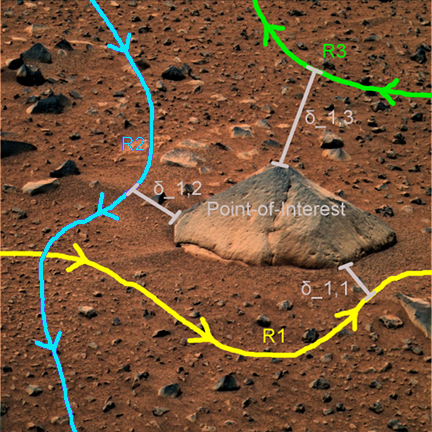
\includegraphics[width=\textwidth]{knudson-fig-2}
\end{column}
\begin{column}{0.3\textwidth}
\caption{
Figure 2 from \cite{knudson2010coevolution}.
}
\end{column}
\end{columns}
\end{figure}

\end{frame}

\begin{frame}{Treatments}
\Large
\begin{itemize}
\item system
\begin{itemize}
\item selection $\sim$ group performance
\end{itemize}
\item local
\begin{itemize}
\item selection $\sim$ \# waypoints an individual visited
\end{itemize}
\item difference
\begin{itemize}
\item selection $\sim$ group performance $-$ group performance w/o individual
\end{itemize}
\item random
\begin{itemize}
\item control treatment
\end{itemize}
\end{itemize}

\end{frame}

\begin{frame}{Results}

\begin{figure}

\begin{columns}
\begin{column}{0.7\textwidth}
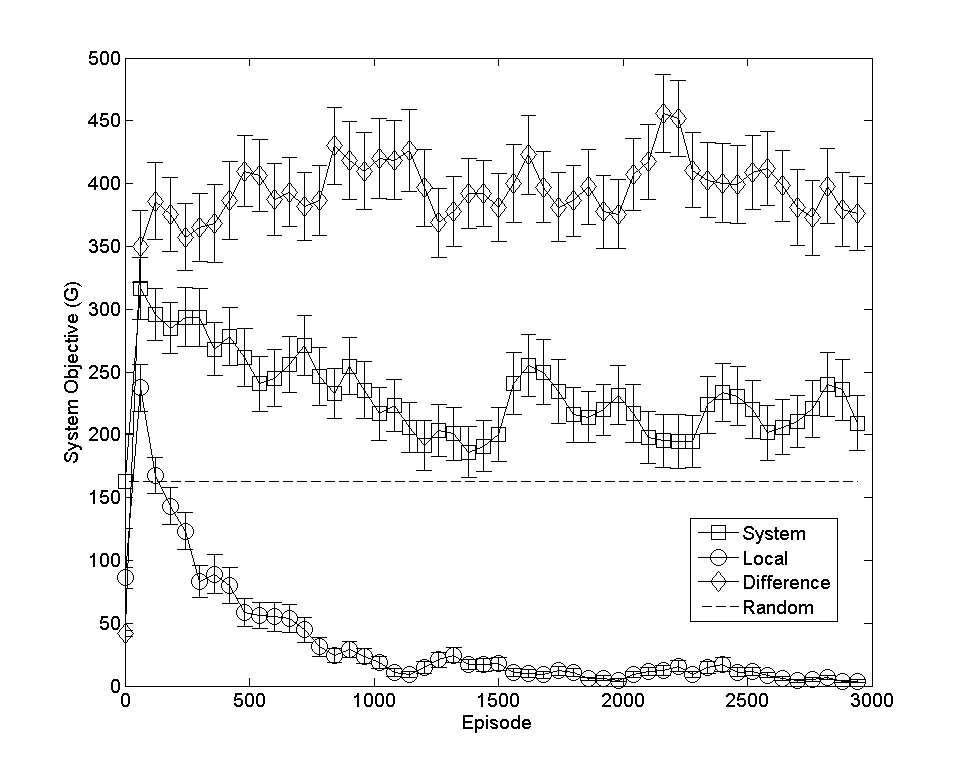
\includegraphics[width=\textwidth]{knudson-fig-7-a}
\end{column}
\begin{column}{0.3\textwidth}
\caption{
Left column of Figure 7 from \cite{knudson2010coevolution}.
}
\end{column}
\end{columns}

\end{figure}

\end{frame}

\begin{frame}{Results}

\begin{figure}

\begin{columns}
\begin{column}{0.7\textwidth}
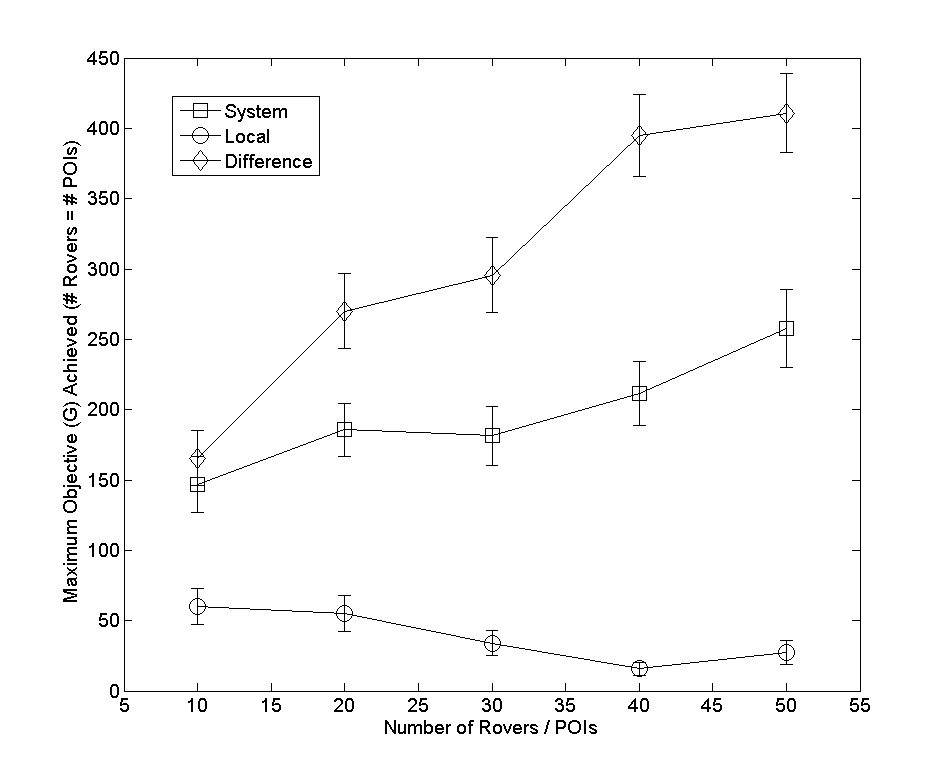
\includegraphics[width=\textwidth]{knudson-fig-7-b}
\end{column}
\begin{column}{0.3\textwidth}
\caption{
Right column of Figure 7 from \cite{knudson2010coevolution}.
}
\end{column}
\end{columns}

\end{figure}

\end{frame}

\begin{frame}{Discussion}

difference metric is (in principle) generalizable to other problem domains

however, with large groups and without shortcuts it could become computationally prohibitive

assumption for shortcut:
effect of agent on other agents is negligible compared to direct effect of agent on objective

concern:
difference metric might break down in some cases with extreme specialization
\begin{itemize}
\item specifically, when team performance is varyingly sensitive to different team roles 
\end{itemize}


\end{frame}

\begin{frame}{Discussion}

How much does team score decrease when removing a sweeper versus removing the thrower?

\begin{figure}
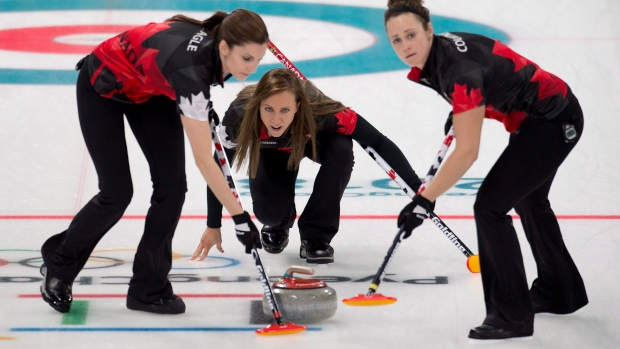
\includegraphics[width=\textwidth]{curling-team}
\caption{A curling team in action.}
\label{fig:curling-team}
\end{figure}

\end{frame}
